% =====================================================================
% File        : indexing_matrix_matlab.tex
% Deskripsi   : Indexing Matrix in MATLAB: magic(), indexing, eye/triu/tril, sum()
%               dengan contoh A = magic(4)
% =====================================================================
\documentclass[aspectratio=169,11pt]{beamer}
\usetheme{metropolis}
\usepackage[utf8]{inputenc}
\usepackage{amsmath,amssymb}
\usepackage{booktabs}
\usepackage{listings}
\usepackage{tikz}
\usetikzlibrary{matrix,positioning,arrows.meta,fit,calc}

% Matriks A = magic(4) dengan label indeks baris/kolom; #1 = anotasi tambahan
\newcommand{\Amat}[1]{%
\begin{tikzpicture}
\matrix (m) [matrix of math nodes, ampersand replacement=\&,
             nodes={minimum width=2.8em, minimum height=1.7em},
             left delimiter={[}, right delimiter={]}]
{ 16 \& 2 \& 3 \& 13\\
  5 \& 11 \& 10 \& 8\\
  9 \& 7 \& 6 \& 12\\
  4 \& 14 \& 15 \& 1\\ };
\foreach \c in {1,...,4}
  \node[font=\scriptsize, text=gray] at ([yshift=8pt]m-1-\c.north) {\c};
\foreach \r in {1,...,4}
  \node[font=\scriptsize, text=gray] at ([xshift=-16pt]m-\r-1.west) {\r};
#1
\end{tikzpicture}}

\definecolor{kolom}{RGB}{31,119,180}
\definecolor{baris}{RGB}{214,39,40}
\definecolor{kode}{RGB}{245,245,245}
\newcommand{\z}{\textcolor{gray!45}{0}}

\lstset{
  language=Matlab,
  basicstyle=\ttfamily\small,
  backgroundcolor=\color{kode},
  keywordstyle=\color{kolom}\bfseries,
  commentstyle=\color{gray}\itshape,
  frame=single, rulecolor=\color{gray!40},
  columns=fullflexible, keepspaces=true,
  xleftmargin=4pt, xrightmargin=4pt
}

\title{Indexing Matrix in MATLAB}
\subtitle{\texttt{magic()}, akses elemen, \texttt{eye}/\texttt{triu}/\texttt{tril}, dan \texttt{sum()}}
\author{Andreas Syaloom Kurniawan}
\institute{Faculty of Economics and Business, Universitas Gadjah Mada}
\date{}

\begin{document}

\maketitle

% ---------------------------------------------------------------------
\begin{frame}{Apa itu \texttt{magic(n)}?}
\texttt{magic(n)} menghasilkan \alert{magic square} berukuran $n\times n$:
\begin{itemize}
  \item berisi bilangan bulat $1, 2, \dots, n^2$, masing-masing tepat sekali;
  \item jumlah setiap \textbf{baris}, setiap \textbf{kolom}, dan kedua
        \textbf{diagonal} utama sama besar.
\end{itemize}
\vspace{0.5em}
Konstanta ajaibnya:
\[
  S(n) = \frac{n(n^2+1)}{2}
  \qquad\Longrightarrow\qquad
  S(4) = \frac{4(16+1)}{2} = 34
\]
\vspace{0.3em}
\small Catatan: valid untuk $n\ge 3$. Di MATLAB fungsi ini terutama dipakai
sebagai \emph{matriks uji} yang deterministik.
\end{frame}

% ---------------------------------------------------------------------
\begin{frame}[fragile]{Contoh: \texttt{A = magic(4)}}
\begin{columns}[T]
\column{0.45\textwidth}
\begin{lstlisting}
>> A = magic(4)
A =
    16     2     3    13
     5    11    10     8
     9     7     6    12
     4    14    15     1
\end{lstlisting}
\column{0.5\textwidth}
\[
A=\begin{bmatrix}
16 & 2 & 3 & 13\\
5 & 11 & 10 & 8\\
9 & 7 & 6 & 12\\
4 & 14 & 15 & 1
\end{bmatrix}
\]
\begin{itemize}\small
  \item Ukuran: $4\times 4$, isi $1,\dots,16$
  \item Setiap baris/kolom/diagonal berjumlah $34$
\end{itemize}
\end{columns}
\end{frame}

% ---------------------------------------------------------------------
\begin{frame}[fragile]{Akses elemen: \texttt{A(baris,kolom)}}
\begin{columns}[c]
\column{0.48\textwidth}
\centering
\Amat{
  \node[draw=baris, very thick, rounded corners, inner sep=0pt, fit=(m-1-3)] {};
  \node[draw=teal, very thick, rounded corners, inner sep=0pt, fit=(m-4-4)] {};
}

\scriptsize\textcolor{gray}{angka abu-abu = nomor baris/kolom}
\column{0.48\textwidth}
\small
Format umum: \texttt{A(\textcolor{baris}{i},\textcolor{kolom}{j})} = elemen
di baris $i$, kolom $j$.
\begin{lstlisting}[basicstyle=\ttfamily\footnotesize]
>> A(1,3)        % baris 1, kolom 3
ans = 3
>> A(end,end)    % elemen terakhir
ans = 1
\end{lstlisting}
\texttt{end} = indeks terakhir pada dimensi tempat ia ditulis. Untuk $A$
$4\times4$: \texttt{A(end,end)} $\equiv$ \texttt{A(4,4)}.
\end{columns}
\end{frame}

% ---------------------------------------------------------------------
\begin{frame}[fragile]{Akses satu kolom atau satu baris: titik dua \texttt{:}}
\begin{columns}[c]
\column{0.48\textwidth}
\centering
\Amat{
  \node[draw=kolom, very thick, rounded corners, inner sep=1pt, fit=(m-1-3)(m-4-3)] {};
  \node[draw=baris, very thick, rounded corners, inner sep=1pt, fit=(m-2-1)(m-2-4)] {};
}
\column{0.48\textwidth}
\small
\texttt{:} sendirian = \alert{semua indeks} pada dimensi itu.
\begin{lstlisting}[basicstyle=\ttfamily\scriptsize]
>> A(:,3)     % semua baris, kolom 3
ans =
     3
    10
     6
    15
>> A(2,:)     % baris 2, semua kolom
ans =
     5    11    10     8
\end{lstlisting}
Hasil: kolom $4\times1$, baris $1\times4$.
\end{columns}
\end{frame}

% ---------------------------------------------------------------------
\begin{frame}[fragile]{Linear indexing: \texttt{A(3)}}
\begin{columns}[c]
\column{0.48\textwidth}
\centering
\Amat{
  \foreach \r in {1,...,4}{
    \foreach \c in {1,...,4}{
      \pgfmathtruncatemacro{\k}{\r+(\c-1)*4}
      \node[font=\tiny, text=kolom, anchor=north east, inner sep=1pt]
            at (m-\r-\c.north east) {\k};
    }
  }
  \node[draw=baris, very thick, rounded corners, inner sep=0pt, fit=(m-3-1)] {};
}

\scriptsize\textcolor{kolom}{angka kecil biru = urutan linear}
\column{0.48\textwidth}
\small
Dengan \textbf{satu} indeks, MATLAB membaca matriks
\alert{kolom demi kolom} (\emph{column-major}):
\begin{lstlisting}[basicstyle=\ttfamily\footnotesize]
>> A(3)        % elemen ke-3
ans = 9
>> A(3,1)      % sama persis
ans = 9
\end{lstlisting}
Untuk matriks $m\times n$:
\[
  \texttt{A(i,j)} = \texttt{A}\big(i + (j-1)\,m\big)
\]
Contoh: \texttt{A(1,3)} = \texttt{A(1+2*4)} = \texttt{A(9)} = 3.
\end{columns}
\end{frame}

% ---------------------------------------------------------------------
\begin{frame}[fragile]{Rentang indeks: \texttt{A(3:end,2)}}
\begin{columns}[c]
\column{0.48\textwidth}
\centering
\Amat{
  \node[draw=kolom, very thick, rounded corners, inner sep=1pt, fit=(m-3-2)(m-4-2)] {};
}
\column{0.48\textwidth}
\small
\texttt{a:b} = indeks $a, a+1, \dots, b$.
\begin{lstlisting}[basicstyle=\ttfamily\footnotesize]
>> A(3:end,2)  % baris 3..akhir
ans =
     7
    14
>> A(1:2,2:3)  % sub-matriks 2x2
ans =
     2     3
    11    10
\end{lstlisting}
\textcolor{baris}{\textbf{Jebakan}}: \texttt{A(3:,2)} \alert{error} karena
rentang wajib punya batas akhir. Tulis \texttt{A(3:end,2)}.
\end{columns}
\end{frame}

% ---------------------------------------------------------------------
\begin{frame}[fragile]{Membuat matriks identitas: \texttt{eye(n)}}
\begin{columns}[c]
\column{0.45\textwidth}
\centering
\[
\texttt{eye(4)} =
\begin{bmatrix}
1 & \z & \z & \z\\
\z & 1 & \z & \z\\
\z & \z & 1 & \z\\
\z & \z & \z & 1
\end{bmatrix}
\]
\small Diagonal utama $=1$, sisanya $0$.
\column{0.51\textwidth}
\begin{lstlisting}[basicstyle=\ttfamily\footnotesize]
>> I = eye(4)       % identitas 4x4
>> eye(2,3)         % 2x3, diagonal 1
ans =
     1     0     0
     0     1     0
>> isequal(A*eye(4), A)
ans = 1
\end{lstlisting}
\small
Sifat: $AI = IA = A$. Berguna misalnya untuk $(X'X + \lambda I)$
pada regresi ridge.
\end{columns}
\end{frame}

% ---------------------------------------------------------------------
\begin{frame}[fragile]{Segitiga atas \texttt{triu} dan segitiga bawah \texttt{tril}}
\centering
\[
\texttt{triu(A)} =
\begin{bmatrix}
16 & 2 & 3 & 13\\
\z & 11 & 10 & 8\\
\z & \z & 6 & 12\\
\z & \z & \z & 1
\end{bmatrix}
\qquad
\texttt{tril(A)} =
\begin{bmatrix}
16 & \z & \z & \z\\
5 & 11 & \z & \z\\
9 & 7 & 6 & \z\\
4 & 14 & 15 & 1
\end{bmatrix}
\]
\begin{lstlisting}[basicstyle=\ttfamily\footnotesize]
>> triu(A)   % u = upper: diagonal dan di ATAS-nya dipertahankan
>> tril(A)   % l = lower: diagonal dan di BAWAH-nya dipertahankan
\end{lstlisting}
\small Elemen lainnya diganti $0$; ukuran matriks tetap $4\times4$.
\end{frame}

% ---------------------------------------------------------------------
\begin{frame}[fragile]{Geser diagonal dengan argumen \texttt{k}, dan trik cepat}
\begin{columns}[T]
\column{0.5\textwidth}
\centering
\[
\texttt{triu(A,1)} =
\begin{bmatrix}
\z & 2 & 3 & 13\\
\z & \z & 10 & 8\\
\z & \z & \z & 12\\
\z & \z & \z & \z
\end{bmatrix}
\]
\small \texttt{k = 1}: mulai satu di atas diagonal (diagonal ikut nol).\\
\texttt{tril(A,-1)}: mulai satu di bawah diagonal.
\column{0.46\textwidth}
\begin{lstlisting}[basicstyle=\ttfamily\footnotesize]
>> triu(ones(4))  % isi 1
ans =
     1     1     1     1
     0     1     1     1
     0     0     1     1
     0     0     0     1
>> isequal(tril(A) + triu(A,1), A)
ans = 1
\end{lstlisting}
\small Dekomposisi: $A = \texttt{tril(A)} + \texttt{triu(A,1)}$.
\end{columns}
\end{frame}

% ---------------------------------------------------------------------
\begin{frame}[fragile]{Apa itu \texttt{sum()}?}
\begin{lstlisting}
S = sum(A)          % default: jumlah per kolom (untuk matriks)
S = sum(A, dim)     % jumlahkan sepanjang dimensi ke-dim
S = sum(A, 'all')   % jumlah seluruh elemen
\end{lstlisting}
\vspace{0.4em}
Argumen \texttt{dim} adalah \alert{nomor dimensi (sumbu)} yang
``dilipat'' saat penjumlahan:
\[
  \texttt{sum(A,1)}_j = \sum_{i=1}^{m} a_{ij},
  \qquad
  \texttt{sum(A,2)}_i = \sum_{j=1}^{n} a_{ij}
\]
Dimensi yang dijumlahkan menyusut menjadi berukuran $1$.
\end{frame}

% ---------------------------------------------------------------------
\begin{frame}{Arti argumen \texttt{dim} (untuk $A$ berukuran $4\times4$)}
\centering
\renewcommand{\arraystretch}{1.3}
\begin{tabular}{c l l}
\toprule
\texttt{dim} & Sumbu & Arti untuk $A$ $4\times4$ \\
\midrule
1 & baris (vertikal, ke bawah)        & jumlah per \textcolor{kolom}{kolom} $\rightarrow 1\times4$ \\
2 & kolom (horizontal, ke kanan)      & jumlah per \textcolor{baris}{baris} $\rightarrow 4\times1$ \\
3 & ``halaman'' (kedalaman, array 3-D) & ukurannya 1 $\rightarrow$ hasil $= A$ \\
\bottomrule
\end{tabular}

\vspace{1em}
\small\raggedright
MATLAB memandang $A$ sebagai array berukuran $4\times4\times1\times1\times\cdots$.
Karena itu \texttt{dim} $\ge 3$ (misalnya 3, 5, 7) tidak error, tetapi
hasilnya identik dengan $A$.
\end{frame}

% ---------------------------------------------------------------------
\begin{frame}[fragile]{\texttt{sum(A,1)}: jumlah per kolom}
\begin{columns}[c]
\column{0.5\textwidth}
\centering
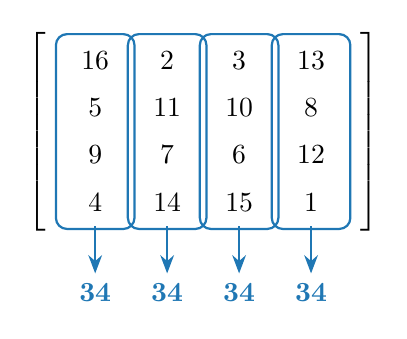
\begin{tikzpicture}
\matrix (m) [matrix of math nodes, nodes={minimum width=2.6em, minimum height=1.7em},
             left delimiter={[}, right delimiter={]}]
{ 16 & 2 & 3 & 13\\
  5 & 11 & 10 & 8\\
  9 & 7 & 6 & 12\\
  4 & 14 & 15 & 1\\ };
\foreach \c in {1,...,4}{
  \node[draw=kolom, thick, rounded corners, inner sep=1pt,
        fit=(m-1-\c)(m-4-\c)] {};
  \draw[-{Stealth}, kolom, thick] (m-4-\c.south) -- ++(0,-0.6)
        node[below, text=kolom, font=\bfseries] {34};
}
\end{tikzpicture}
\column{0.45\textwidth}
\small
Kolom 1: $16+5+9+4 = 34$\\
Kolom 2: $2+11+7+14 = 34$\\
Kolom 3: $3+10+6+15 = 34$\\
Kolom 4: $13+8+12+1 = 34$
\begin{lstlisting}
>> sum(A,1)
ans =
    34    34    34    34
\end{lstlisting}
Hasil: vektor \textbf{baris} $1\times4$.
\end{columns}
\end{frame}

% ---------------------------------------------------------------------
\begin{frame}[fragile]{\texttt{sum(A,2)}: jumlah per baris}
\begin{columns}[c]
\column{0.5\textwidth}
\centering
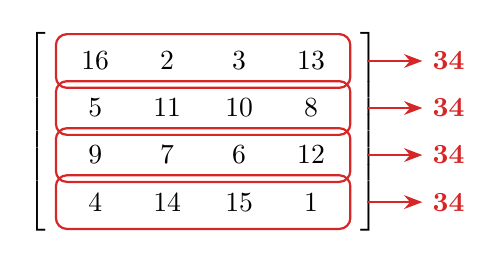
\begin{tikzpicture}
\matrix (m) [matrix of math nodes, nodes={minimum width=2.6em, minimum height=1.7em},
             left delimiter={[}, right delimiter={]}]
{ 16 & 2 & 3 & 13\\
  5 & 11 & 10 & 8\\
  9 & 7 & 6 & 12\\
  4 & 14 & 15 & 1\\ };
\foreach \r in {1,...,4}{
  \node[draw=baris, thick, rounded corners, inner sep=1pt,
        fit=(m-\r-1)(m-\r-4)] {};
  \draw[-{Stealth}, baris, thick] (m-\r-4.east) ++(0.25,0) -- ++(0.7,0)
        node[right, text=baris, font=\bfseries] {34};
}
\end{tikzpicture}
\column{0.45\textwidth}
\small
Baris 1: $16+2+3+13 = 34$\\
Baris 2: $5+11+10+8 = 34$\\
Baris 3: $9+7+6+12 = 34$\\
Baris 4: $4+14+15+1 = 34$
\begin{lstlisting}
>> sum(A,2)
ans =
    34
    34
    34
    34
\end{lstlisting}
Hasil: vektor \textbf{kolom} $4\times1$.
\end{columns}
\end{frame}

% ---------------------------------------------------------------------
\begin{frame}[fragile]{\texttt{sum(A,'all')}: jumlah seluruh elemen}
\begin{columns}[c]
\column{0.5\textwidth}
\centering
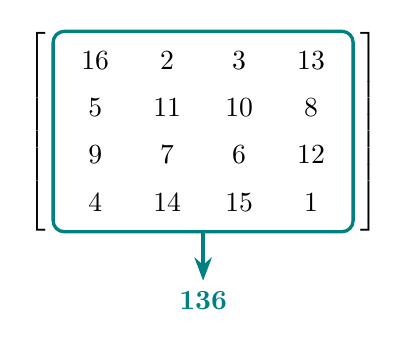
\begin{tikzpicture}
\matrix (m) [matrix of math nodes, nodes={minimum width=2.6em, minimum height=1.7em},
             left delimiter={[}, right delimiter={]}]
{ 16 & 2 & 3 & 13\\
  5 & 11 & 10 & 8\\
  9 & 7 & 6 & 12\\
  4 & 14 & 15 & 1\\ };
\node[draw=teal, very thick, rounded corners, inner sep=2pt,
      fit=(m-1-1)(m-4-4)] (all) {};
\draw[-{Stealth}, teal, very thick] (all.south) -- ++(0,-0.6)
      node[below, text=teal, font=\bfseries] {136};
\end{tikzpicture}
\column{0.45\textwidth}
\small
Semua dimensi dilipat sekaligus, sehingga hasilnya \textbf{skalar} $1\times1$:
\[
  \texttt{sum(A,'all')} = \sum_{i=1}^{4}\sum_{j=1}^{4} a_{ij} = 136
\]
\begin{lstlisting}
>> sum(A,'all')  % 136
>> sum(A,[1 2])  % vecdim
>> sum(sum(A))   % dua tahap
>> sum(A(:))     % vektorisasi
\end{lstlisting}
Cek: $4\times34 = 136 = \dfrac{16\cdot17}{2}$.
\end{columns}
\end{frame}

% ---------------------------------------------------------------------
\begin{frame}[fragile]{\texttt{sum(B,[1,2])} dengan \texttt{B = magic(5)}: kenapa 325?}
\begin{columns}[c]
\column{0.52\textwidth}
\centering
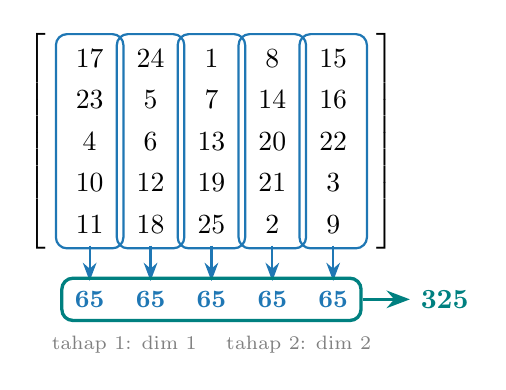
\begin{tikzpicture}
\matrix (m) [matrix of math nodes, nodes={minimum width=2.2em, minimum height=1.5em},
             left delimiter={[}, right delimiter={]}]
{ 17 & 24 & 1 & 8 & 15\\
  23 & 5 & 7 & 14 & 16\\
  4 & 6 & 13 & 20 & 22\\
  10 & 12 & 19 & 21 & 3\\
  11 & 18 & 25 & 2 & 9\\ };
\foreach \c in {1,...,5}{
  \node[draw=kolom, thick, rounded corners, inner sep=1pt,
        fit=(m-1-\c)(m-5-\c)] {};
  \draw[-{Stealth}, kolom, thick] (m-5-\c.south) -- ++(0,-0.45)
        node[below, text=kolom, font=\bfseries\small] (s\c) {65};
}
\node[draw=teal, very thick, rounded corners, inner sep=1pt, fit=(s1)(s5)] (row) {};
\draw[-{Stealth}, teal, very thick] (row.east) -- ++(0.6,0)
      node[right, text=teal, font=\bfseries] {325};
\node[below=0.05 of row, font=\scriptsize, text=gray] {tahap 1: dim 1 \quad tahap 2: dim 2};
\end{tikzpicture}
\column{0.44\textwidth}
\small
\texttt{[1,2]} = daftar dimensi yang \alert{semuanya} dilipat:
\begin{lstlisting}[basicstyle=\ttfamily\footnotesize]
>> sum(B,1)        % 1x5: 65 semua
>> sum(sum(B,1),2) % 325
>> sum(B,[1,2])    % 325
\end{lstlisting}
Setelah dimensi 1 dilipat masih ada \textbf{lima} angka 65:
\[
  65\times5 = 325 = \frac{25\cdot26}{2}
\]
\textcolor{baris}{Bukan} $65+65=130$: itu sama dengan satu baris + satu kolom, bukan operasi \texttt{sum} mana pun.
\end{columns}
\end{frame}

% ---------------------------------------------------------------------
\begin{frame}[fragile]{Menjumlahkan baris 1 dan 2 saja: \texttt{B(1:2,:)}}
\begin{columns}[c]
\column{0.5\textwidth}
\centering
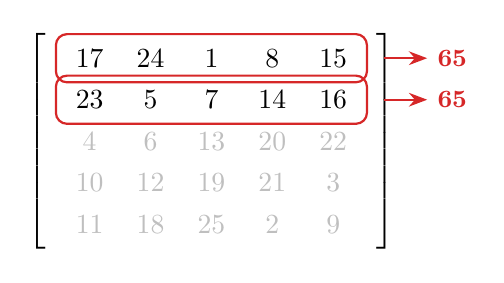
\begin{tikzpicture}
\matrix (m) [matrix of math nodes, nodes={minimum width=2.2em, minimum height=1.5em},
             left delimiter={[}, right delimiter={]},
             row 3/.style={nodes={text=gray!50}},
             row 4/.style={nodes={text=gray!50}},
             row 5/.style={nodes={text=gray!50}}]
{ 17 & 24 & 1 & 8 & 15\\
  23 & 5 & 7 & 14 & 16\\
  4 & 6 & 13 & 20 & 22\\
  10 & 12 & 19 & 21 & 3\\
  11 & 18 & 25 & 2 & 9\\ };
\foreach \r in {1,2}{
  \node[draw=baris, thick, rounded corners, inner sep=1pt,
        fit=(m-\r-1)(m-\r-5)] {};
  \draw[-{Stealth}, baris, thick] (m-\r-5.east) ++(0.25,0) -- ++(0.55,0)
        node[right, text=baris, font=\bfseries\small] {65};
}
\end{tikzpicture}

\vspace{0.3em}
\small Indexing: \texttt{B(\alert{1:2},:)} = baris 1--2, semua kolom
\column{0.46\textwidth}
\begin{lstlisting}[basicstyle=\ttfamily\footnotesize]
>> sum(B(1:2,:), 2)    % tiap baris
ans =
    65
    65
>> sum(B(1:2,:), 'all') % total
ans = 130
>> sum(B(1:2,:), 1)    % per elemen
ans =
  40  29   8  22  31
\end{lstlisting}
\small Baris ke-3 sampai ke-5 tidak ikut dihitung.
\end{columns}
\end{frame}

% ---------------------------------------------------------------------
\begin{frame}[fragile]{Menjumlahkan kolom 1 dan 2 saja: \texttt{B(:,1:2)}}
\begin{columns}[c]
\column{0.5\textwidth}
\centering
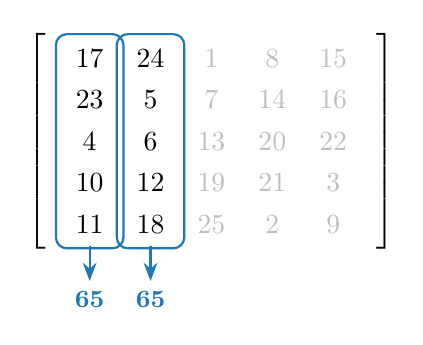
\begin{tikzpicture}
\matrix (m) [matrix of math nodes, nodes={minimum width=2.2em, minimum height=1.5em},
             left delimiter={[}, right delimiter={]},
             column 3/.style={nodes={text=gray!50}},
             column 4/.style={nodes={text=gray!50}},
             column 5/.style={nodes={text=gray!50}}]
{ 17 & 24 & 1 & 8 & 15\\
  23 & 5 & 7 & 14 & 16\\
  4 & 6 & 13 & 20 & 22\\
  10 & 12 & 19 & 21 & 3\\
  11 & 18 & 25 & 2 & 9\\ };
\foreach \c in {1,2}{
  \node[draw=kolom, thick, rounded corners, inner sep=1pt,
        fit=(m-1-\c)(m-5-\c)] {};
  \draw[-{Stealth}, kolom, thick] (m-5-\c.south) -- ++(0,-0.45)
        node[below, text=kolom, font=\bfseries\small] {65};
}
\end{tikzpicture}

\small Indexing: \texttt{B(:,\alert{1:2})} = semua baris, kolom 1--2
\column{0.46\textwidth}
\begin{lstlisting}[basicstyle=\ttfamily\footnotesize]
>> sum(B(:,1:2), 1)    % tiap kolom
ans =
    65    65
>> sum(B(:,1:2), 'all') % total
ans = 130
>> sum(B(:,1:2), 2)'   % per elemen
ans =
  41  28  10  22  29
\end{lstlisting}
\small Tanda \texttt{'} hanya mentranspos hasil $5\times1$ agar ringkas.
Kolom ke-3 sampai ke-5 tidak ikut dihitung.
\end{columns}
\end{frame}

% ---------------------------------------------------------------------
\begin{frame}[fragile]{Indexing tidak berurutan dan jebakan \texttt{B(1,2)}}
\textbf{Baris/kolom tidak berurutan}: pakai vektor indeks.
\begin{lstlisting}[basicstyle=\ttfamily\footnotesize]
>> sum(B([1 3],:), 'all')   % baris 1 dan 3  -> 130
>> sum(B(:,[2 5]), 'all')   % kolom 2 dan 5  -> 130
\end{lstlisting}
\textbf{Jebakan}: koma memisahkan \emph{baris} dan \emph{kolom}, bukan daftar baris.
\begin{columns}[T]
\column{0.48\textwidth}
\begin{lstlisting}[basicstyle=\ttfamily\footnotesize]
>> B(1,2)      % SATU elemen -> 24
>> B([1 2],:)  % baris 1 DAN 2 (2x5)
\end{lstlisting}
\column{0.48\textwidth}
\footnotesize
\renewcommand{\arraystretch}{1.1}
\begin{tabular}{l l}
\toprule
Ekspresi & Artinya \\
\midrule
\texttt{B(i,:)} & seluruh baris ke-$i$ \\
\texttt{B(:,j)} & seluruh kolom ke-$j$ \\
\texttt{B(i,j)} & satu elemen \\
\texttt{B([i k],:)} & beberapa baris \\
\texttt{B(:,[j l])} & beberapa kolom \\
\bottomrule
\end{tabular}
\end{columns}
\end{frame}

% ---------------------------------------------------------------------
\begin{frame}[fragile]{Pelengkap: \texttt{dim} $\ge 3$}
\begin{lstlisting}
>> isequal(sum(A,3), A)
ans = 1
>> isequal(sum(A,7), A)
ans = 1
\end{lstlisting}
\small Dimensi ke-3 dst.\ berukuran 1, jadi tidak ada yang dijumlahkan.
Dimensi ini baru bermakna kalau datanya memang array 3-D:
\vspace{0.5em}
\begin{lstlisting}
>> B = cat(3, A, 2*A);   % size 4x4x2
>> sum(B,3)              % = A + 2*A = 3*A
\end{lstlisting}
\end{frame}

% ---------------------------------------------------------------------
\begin{frame}[fragile]{Hasil indexing juga matriks}
\begin{columns}[T]
\column{0.5\textwidth}
\small
Di MATLAB semua data numerik adalah \alert{array}. Skalar dan vektor
hanyalah matriks dengan ukuran khusus.
\vspace{0.4em}

\footnotesize
\renewcommand{\arraystretch}{1.15}
\begin{tabular}{l c l}
\toprule
Ekspresi & \texttt{size} & Jenis \\
\midrule
\texttt{A(1,3)}     & $1\times1$ & skalar \\
\texttt{A(:,3)}     & $4\times1$ & vektor kolom \\
\texttt{A(2,:)}     & $1\times4$ & vektor baris \\
\texttt{A(1:2,2:3)} & $2\times2$ & sub-matriks \\
\bottomrule
\end{tabular}
\column{0.46\textwidth}
\begin{lstlisting}[basicstyle=\ttfamily\footnotesize]
>> class(A(1,3))
ans = 'double'
>> A(:,3)' * A(:,3)
ans = 370   % bisa dioperasikan
\end{lstlisting}
\small \textbf{Salinan, bukan \emph{view}}:
\begin{lstlisting}[basicstyle=\ttfamily\footnotesize]
>> x = A(:,3);
>> x(1) = 100;    % A tetap
>> A(1,3) = 100;  % A berubah
\end{lstlisting}
\scriptsize Berbeda dengan NumPy, di mana slicing menghasilkan \emph{view}.
\end{columns}
\end{frame}

% ---------------------------------------------------------------------
\begin{frame}{Ringkasan}
\begin{itemize}
  \item \texttt{magic(n)}: matriks $n\times n$ berisi $1,\dots,n^2$ dengan jumlah
        baris, kolom, dan diagonal sama, yaitu $n(n^2+1)/2$.
  \item \texttt{sum(A,dim)}: \texttt{dim} adalah \alert{nomor sumbu} yang dijumlahkan.
  \item \texttt{sum(A,1)} $\rightarrow$ per kolom ($1\times n$);\;
        \texttt{sum(A,2)} $\rightarrow$ per baris ($m\times1$).
  \item \texttt{dim} $\ge 3$ pada matriks 2-D mengembalikan $A$ itu sendiri.
  \item Untuk $A=\texttt{magic(4)}$: semua jumlah kolom dan baris $=34$,
        total seluruh elemen $=136$.
\end{itemize}
\end{frame}

\end{document}
